\documentclass[12pt]{report} % \documentclass[12pt, demo]{report} -> speed up (no image load)

\usepackage{amsthm}
\usepackage{amsmath}
\usepackage{amssymb}
\usepackage{graphicx}
\usepackage{subcaption}
\usepackage[a4paper, top=2cm, bottom=2cm, right=2cm, left=3.5cm]{geometry}
\usepackage{pdfpages}
\usepackage{setspace}
\onehalfspacing

\begin{document}

% ufficiale
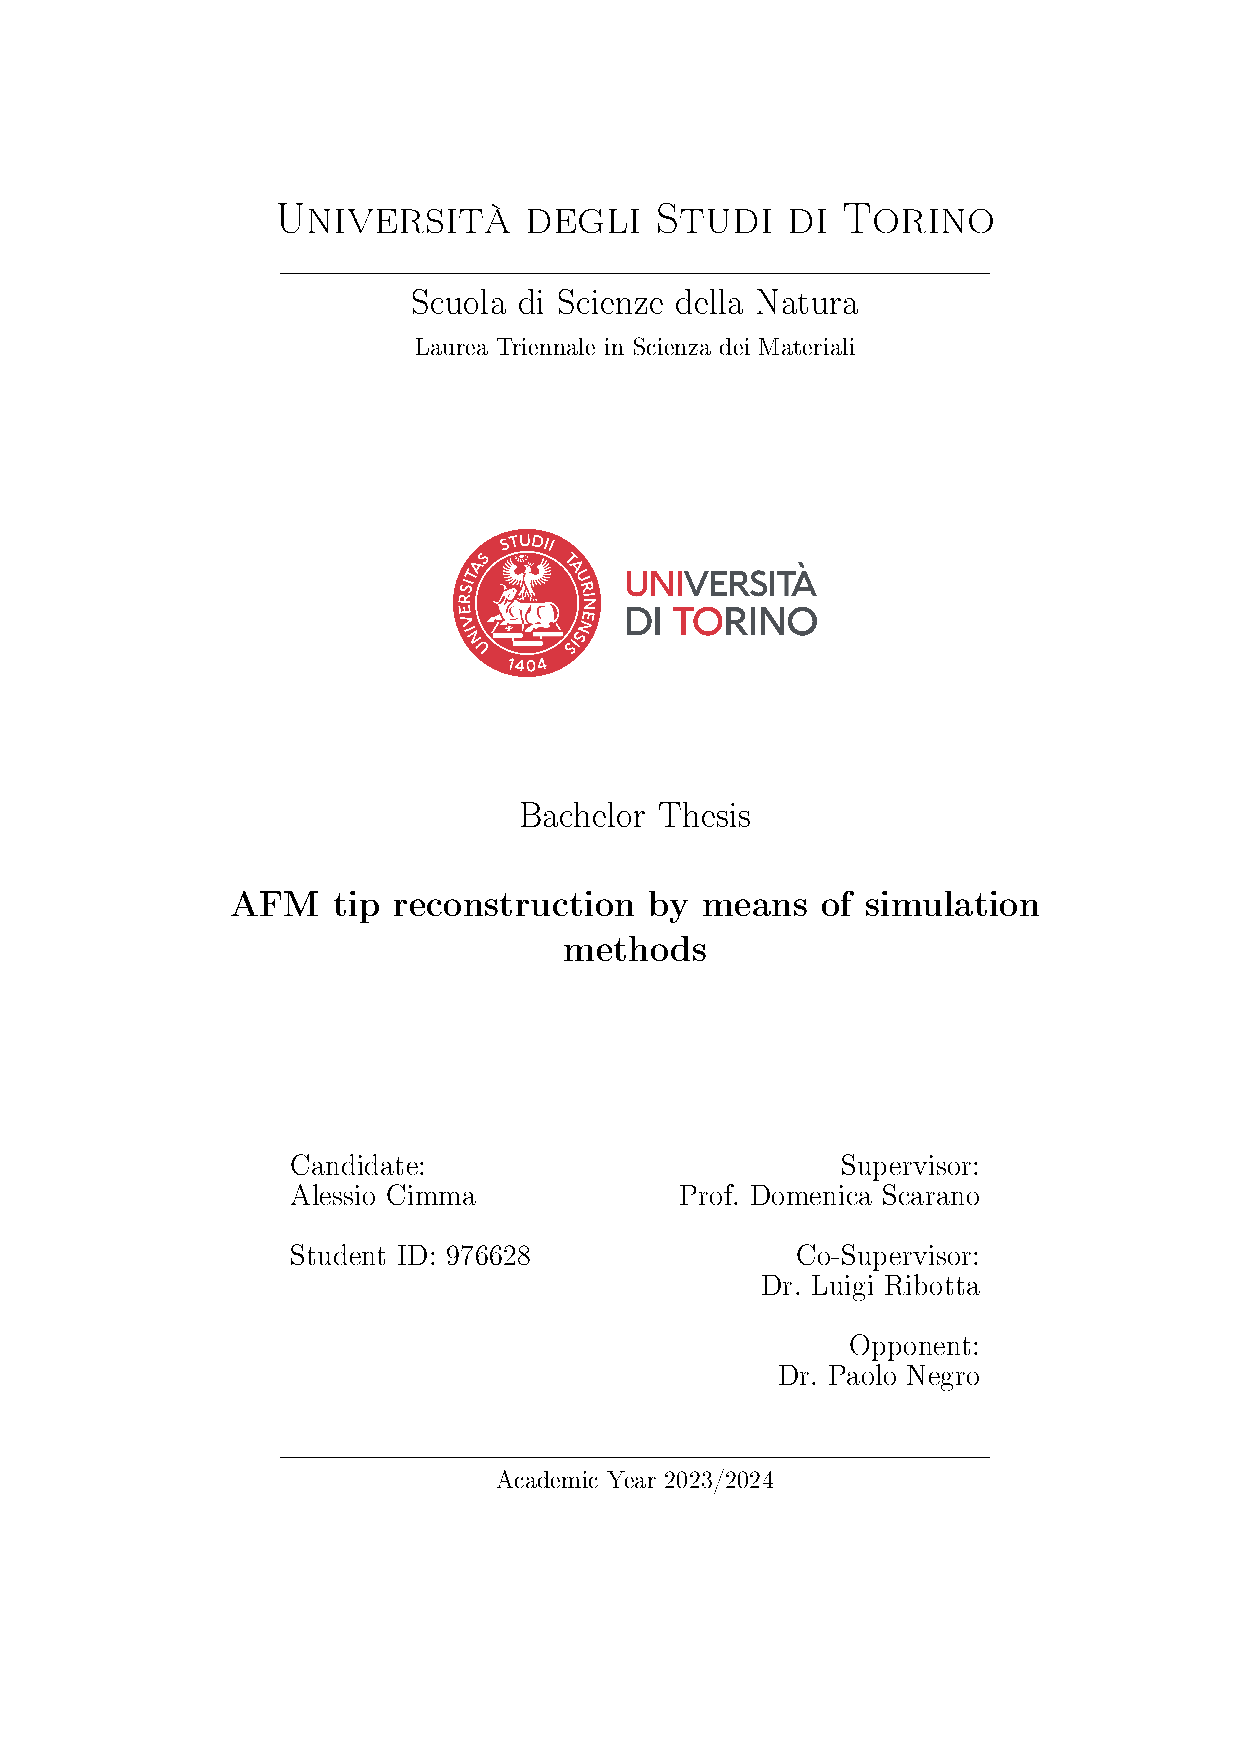
\includepdf[pages={1}]{./frontespizio.pdf}

\pagenumbering{arabic}
\setcounter{page}{0}
\newpage

\noindent Nanometrology supports nanoscience and nanotechnology in many ways, including the reducing of the measurements uncertainty, the definition of models and methodologies, the traceability of measurements at the nanoscale level, as well as the development of samples and reference materials.

Atomic Force Microscope (AFM) is widely used for 3D topographical measurements at nanometer scale (from 1 nm to 100 nm). AFM images are due to the convolution of the sample and tip shapes, and of the tip-sample-substrate interactions. Therefore, despite the subnanometric accuracy in the vertical direction (Z), the AFM lateral resolution (X and Y directions) is mainly limited by the influence of the tip shape. Hence, it is essential to carry out the accurate tip reconstruction, before analyzing the dimensional and mechanical data of different materials at the nanoscale, such as semiconductors, biological materials (such as scaffold or cells) or inorganic nanoparticles with different size, shape and geometry.

Several methods of AFM tip reconstruction are discussed in literature. This work focuses on the “known tip characteriser” approach, which exploits well-known dimensional and shape parameters from the crystalline structure of a nanoparticle. 

The goal of this study is the development of an innovative approach for the reconstruction of the 3D shape of an AFM tip in a Python module. As starting point, the Python module generates the topography of an ideal nanoparticle starting from its nominal dimensional characteristic or from its crystalline structure. To this goal, a 3D computer graphics software tool, such as Blender, is used to generate a nanoparticle mesh made of triangles. This graphics tool permits also the generation of multiple nanoparticles, with different geometry, different sizes and orientation on the same image. The geometric shapes including spheres, nanosheets, and bipyramids are simulated as tip characterisers, by means of advanced algorithms for image recognition and shape fitting. Starting from the 3D mesh, the ideal 3D topography is obtained by exploiting a ray tracing algorithm. More specifically, a Z-test (or depth-test) technique is used, which relies on quantifying the distance between an object lying on a substrate and a planar camera, from which perpendicular rays directed towards the substrate depart. 

\begin{figure}[h]
    \centering
    % schema_afm
    \includegraphics[width=0.7\textwidth]{./concept.png}
    \caption{RayTracer Z-test method}
\end{figure}

\newpage

\noindent The novelty of this approach is to consider each pixel of the AFM topography as the result of the interaction of the tip apex considered as a monoatomic Dirac’s delta ray and the generated nanoparticle mesh. The constant evolution of performances, due to ever-improving hardware and dedicated programming languages, makes raytracers advantageous, in terms of rendering speed, accuracy, and efficiency, largely driven by the use of powerful graphics processing units (GPUs). The ability to simulate ideal measurements and accurately reconstruct tip shapes by means of ray tracing techniques opens new possibilities for improving the precision and speed of tip reconstruction algorithms in AFM studies.

Once the ideal topography is created, it is compared to the experimental one. For this, a structure fitting algorithm is used to find the best position and parameters of the ideal structure that needs to be fitted under the measured AFM data. The program begins by finding the maximum peaks in the image using a maximum filter. Then it calculates the best parameters of the structure under analysis and generates it in the best position and rotation using the ray tracer pipeline described before.

Before reconstructing the tip, we need to estimate the lateral size of the tip, also called tip matrix size, able to cover the largest feature present in the image. Using a Boolean mask of the measured topography, it is possible to detect the dimensions in X and Y directions of the nanoparticles.

Tip reconstruction is achieved through a naive erosion algorithm based on morphological dilation and erosion principles, applied to both the ideal and real topography data. The mathematical framework transforms the surface to match the true shape of the tip, by subtracting the generated structure from the measured topography. The algorithm's core is a Minkowski subtraction process, that reconstructs the 3D shape of the tip. Finally, the measured topography is eroded by the reconstructed tip.

This thesis successfully demonstrates the 3D reconstruction of a tip by means of spherical nanoparticles, thus showing the potentiality of the ray tracing algorithm implemented in the Python module for more complex geometries, such as $TiO_2$ nanosheets or other nanoparticles of different nature.

\begin{figure}[h]
    \centering
    % schema_afm
    \includegraphics[width=0.825\textwidth]{./punta_cut_finale.png}
    \caption{Reconstructed 3D tip}
\end{figure}

\end{document}